\section{Validating the Generated Code}
\label{sec:validateprodcons}
As a way of reasoning about the correctness of the translation we compare the generated code to the manually translated code in section~\ref{sec:structuralcodegeneration}. Furthermore, we validate the generated code by executing it and monitoring the behaviour. Afterwards, the behaviour is compared with the behaviour of the CPN model, i.e., a simulation of the same scenario in the CPN model.

\subsection{Manually vs. Automatic Generated Code}
In this section we compare the generated Erlang code for the producer-consumer system to the manually translated Erlang code presented in the structural approach in section~\ref{sec:structuralcodegeneration}. 

\begin{verbatim}
- module(producer).
- export([start/2]).
- record(environment, {
        produced_data,
        data}).

start(Produced_data, Data) -> 
    Env = #environment {produced_data = Produced_data,
    data = Data},
    produce_data(Env).

send_data(Env) -> 
    Data = Env#environment.produced_data,
    next_consumer ! {get, self()},
    receive 
        Nextcons -> 
            Nextcons
    end,
    NewEnv = Env#environment {},
    next_consumer ! {set, Nextcons},
    Id1 = Nextcons,
    Receiver1 = list_to_atom("consumer_ID" ++
    integer_to_list(Id1) ++ "_buffer"),
    Receiver1 ! {send, Data},
    produce_data(NewEnv).

produce_data(Env) -> 
    Data = Env#environment.data,
    Pdata = Env#environment.produced_data,
    NewEnv = Env#environment {produced_data = Data,
    data = Data + 2},
    send_data(NewEnv).
\end{verbatim}


In Listing~\ref{list:generatedproducer} the complete unmodified generated code for the \code{producer} process is shown. The first thing we observe is that the module has the same structure as the manually translated code in Listing~\ref{fig:structureproducer} in section~\ref{sec:structuralcodegeneration}, i.e., the same attributes and function declarations. A difference between the two modules is found in the way they receive the next consumer ID. This is done in line 15-18 of Listing~\ref{list:generatedproducer}. The generated code binds the received ID to the variable \code{Nextcons} and then ends the receive expression. The manually translated module has the expressions, which uses the received ID, in the body of the receive expression. This difference does not change the behaviour of the program, the handwritten code just uses a more compact (and perhaps more readable) way of expressing the same behaviour.

The way the two versions build the ID of the receiving process also differs slightly. In the generated version, the integer identifying the receiving process is bound to a variable in line 21. This is done because in the general case the expression on the right hand side can be any expression evaluating to an integer, and binding the value to a variable makes the code more readable. We can also see that the receiver ID has added the extra word "buffer" in the generated version. This is because the generated code uses a \code{buffer} process with added functionality as explained in section~\ref{sec:astest}. This means that the message has to be sent to the buffer of the receiver instead of the receiver itself.

The generated \code{producer} module contains two lines of code which does not influence the behaviour of the program, namely line 19 and line 29 in Listing~\ref{list:generatedproducer}. In line 19 the environment is updated without any changes made, and in line 29 a value from the environment is read into a local variable which is never read. Both these constructs are correct, according to the behaviour of the CPN model. Since they have no effect on the semantics of the program an optimisation or weeding phase between the Erlang syntax tree and the printing of the code could remove them to make the code more readable.

In Listing~\ref{list:generatedconsumer} we find the generated \code{consumer} module. We compare this module to the manually translated code in Listing~\ref{fig:structureconsumer} in section~\ref{sec:structuralcodegeneration}. Again we find that the two modules have the same structure.

\begin{verbatim}
- module(consumer).
- export([start/2]).
- record(environment, {
        received_data,
        buffer}).

start(Received_data, Buffer) -> 
    Env = #environment {received_data = Received_data,
    buffer = Buffer},
    receive_data(Env).

consume_data(Env) -> 
    Data = Env#environment.received_data,
    NewEnv = Env#environment {},
    receive_data(NewEnv).

receive_data(Env) -> 
    Rdata = Env#environment.received_data,
    Buffer = Env#environment.buffer,
    Buffer ! get,
    receive 
        Data -> 
            Data
    end,
    NewEnv = Env#environment {received_data = Data},
    consume_data(NewEnv).
\end{verbatim}


The main difference between the two \code{consumer} modules is that the generated \code{consumer} uses an explicit \code{buffer} process to receive messages. The \code{pid} of the buffer is found in a field in the environment. In Listing~\ref{list:generatedconsumer} we can see the use of the buffer in lines 19-24. First, the ID of the buffer is found in the environment, next a \code{get} message is sent, and then the \code{consumer} process waits to receive the message from the buffer.

\subsection{Testing the Generated Code}
In this section we describe an execution of the generated code and compare it to a simulation of the CPN model. In order to monitor the behaviour of the program we have decorated the generated code with various expressions. We use the Erlang BIF \code{io:format} to print the state of the program to the screen. In order to monitor the behaviour we have also added sleep calls by using the BIF function \code{timer:sleep} given random sleep periods using the BIF function \code{random:uniform}. Before running the program we introduce a \emph{load-balancer}.

\subsubsection{Adding a Load-balancer to the Model}
As mentioned in section \ref{sec:cpn} the shared place \figitem{NextConsumer} in the producer-consumer model is used to determine which consumer to send to next. In Fig.~\ref{fig:loadbalancer} we see a  ProPCPN model of a very simple load-balancer which is used to update which consumer to send to. The process partition contains the process place \figitem{Switching}, the transition \figitem{SwitchConsumer}, and it is connected to the shared place \figitem{NextConsumer}. The function \code{next} ($fn: CONSUMER \rightarrow CONSUMER$) on the output arc from the transition \figitem{SwitchConsumer} to the shared place \figitem{NextConsumer} is defined as:

\begin{verbatim}
fun next(c(n)) = c(3-n);
\end{verbatim}

\noindent
The function pattern matches the index \code{n} of the consumer, and returns a new consumer where the index is switched.

\begin{figure}
\centering
\includegraphics[scale=0.5]{techniques_and_tool/experiments/graphics/loadbalancer.eps}
\caption{The load-balancer added to the producer-consumer model}
\label{fig:loadbalancer}
\end{figure}

\begin{figure}[h!]
\begin{verbatim}
switch_consumer(Env) -> 
    next_consumer ! {get, self()},
    receive 
        Nextcons -> 
            Nextcons
    end,
    NewEnv = Env#environment {},
    next_consumer ! {set, %% next(nextcons)
    undefined},
    switch_consumer(NewEnv).
\end{verbatim}
\end{figure}

The Erlang function generated from the transition \figitem{SwitchConsumer} is shown in Listing~\ref{list:genswitch}. Notice in line 8, that the signature of the function is simply carried along as a comment. This is because we do not parse CPN ML functions, but by making some small modifications we end up with the final \code{switch\_consumer} function shown in Listing~\ref{list:modgenswitch} for the load-balancer. We have removed the empty \code{NewEnv} environment (line 7 in Listing~\ref{list:genswitch}), and added a sleep for half a second (line 8 in Listing~\ref{list:modgenswitch}) such that the \code{next\_consumer} does not switch constantly. 

\begin{figure}[b!]
\begin{verbatim}
switch_consumer(Env) -> 
    next_consumer ! {get, self()},
    receive 
        Nextcons -> 
            Nextcons
    end,
    next_consumer ! {set, 3-Nextcons},
    timer:sleep(500),
    switch_consumer(Env).
\end{verbatim}
\end{figure}




\subsubsection{Executing the Program}
In order to build confidence in the correctness of the generated code we executed it and monitor its behaviour. We have chosen to present some of the message passing from one of those executions in a Message Sequence Chart (MSC) \cite{MSC}. In Fig.~\ref{fig:msc} we see the execution (vertical lines) of the \code{loadbalancer}, \code{next\_consumer}, \code{producer\_1}, \code{producer\_2}, \code{consumer\_1}, and \code{consumer\_2} process instances. The horizontal lines illustrate the message passing between process instances. In the top of the figure we see how \code{producer\_1} starts by requesting which consumer to send to. The messages received indicates that it is \code{consumer\_1}. Since \code{next\_consumer} is a process instance of a shared module it has to be unlocked, and this is why \code{producer\_1} sends back \code{set} a message. Then the produced data is send to \code{consumer\_1}. In the middle of Fig.~\ref{fig:msc} we see how the \code{loadbalancer} changes the \code{next\_consumer} to \code{consumer\_2}. This has the effect that \code{producer\_2} sends the produced data to \code{consumer\_2} as can be seen in the bottom of the figure.

\begin{figure}[b!]
\centering
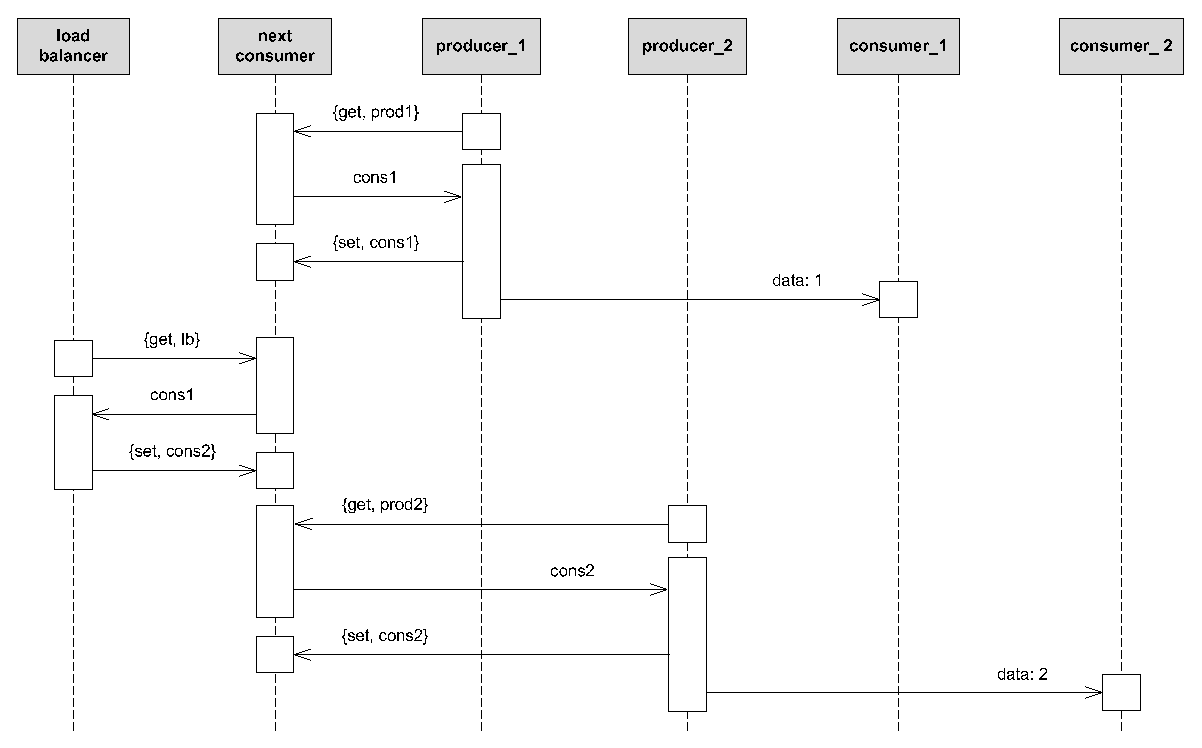
\includegraphics[width=\textwidth]{techniques_and_tool/experiments/graphics/msc.eps}
\caption{A MSC showing part of one of the executions}
\label{fig:msc}
\end{figure}

The behaviour of the generated code can also be simulated in the ProPCPN model. Hence, we have made a simulation in three steps showing the exact same behaviour (a step is a multi-set of binding elements):

\vspace*{1em}
\begin{center}
\begin{tabular}{ccl}
        Step & & Binding element \\  \noalign{\smallskip}\hline\noalign{\smallskip}
	1 & & (\figitem{ProduceData}, \smlbinding{\smlcode{prod=p(1)}, \smlcode{data=1}, \smlcode{pdata=0}}) ++ \\
	  & & (\figitem{SendData}, \smlbinding{\smlcode{prod=p(1)}, \smlcode{data=1}, \smlcode{nextcons=c(1)}}) \\
	2 & & (\figitem{SwitchConsumer}, \smlbinding{\smlcode{nextcons=c(1)}, \smlcode{loadbalancer=lb(1)}}) \\
	3 & & (\figitem{ProduceData}, \smlbinding{\smlcode{prod=p(2)}, \smlcode{data=2}, \smlcode{pdata=0}}) ++ \\
	  & & (\figitem{SendData}, \smlbinding{\smlcode{prod=p(2)}, \smlcode{data=2}, \smlcode{nextcons=c(2)}})
	\\ \noalign{\smallskip}\hline\noalign{\smallskip}
\end{tabular}
\vspace*{1em}
\end{center}

Step one corresponds to the top part of Fig.~\ref{fig:msc} where \code{producer\_1} produces and sends \code{data1} to \code{consumer\_1}. Step two corresponds to the middle of the figure where the \code{loadbalancer} changes the value of \code{next\_consumer}. And finally, step three corresponds to the bottom of the figure where \code{producer\_2} sends \code{data2} to \code{consumer\_2}.
